\documentclass{article}\usepackage[]{graphicx}\usepackage[]{xcolor}
% maxwidth is the original width if it is less than linewidth
% otherwise use linewidth (to make sure the graphics do not exceed the margin)
\makeatletter
\def\maxwidth{ %
  \ifdim\Gin@nat@width>\linewidth
    \linewidth
  \else
    \Gin@nat@width
  \fi
}
\makeatother

\definecolor{fgcolor}{rgb}{0.345, 0.345, 0.345}
\newcommand{\hlnum}[1]{\textcolor[rgb]{0.686,0.059,0.569}{#1}}%
\newcommand{\hlstr}[1]{\textcolor[rgb]{0.192,0.494,0.8}{#1}}%
\newcommand{\hlcom}[1]{\textcolor[rgb]{0.678,0.584,0.686}{\textit{#1}}}%
\newcommand{\hlopt}[1]{\textcolor[rgb]{0,0,0}{#1}}%
\newcommand{\hlstd}[1]{\textcolor[rgb]{0.345,0.345,0.345}{#1}}%
\newcommand{\hlkwa}[1]{\textcolor[rgb]{0.161,0.373,0.58}{\textbf{#1}}}%
\newcommand{\hlkwb}[1]{\textcolor[rgb]{0.69,0.353,0.396}{#1}}%
\newcommand{\hlkwc}[1]{\textcolor[rgb]{0.333,0.667,0.333}{#1}}%
\newcommand{\hlkwd}[1]{\textcolor[rgb]{0.737,0.353,0.396}{\textbf{#1}}}%
\let\hlipl\hlkwb

\usepackage{framed}
\makeatletter
\newenvironment{kframe}{%
 \def\at@end@of@kframe{}%
 \ifinner\ifhmode%
  \def\at@end@of@kframe{\end{minipage}}%
  \begin{minipage}{\columnwidth}%
 \fi\fi%
 \def\FrameCommand##1{\hskip\@totalleftmargin \hskip-\fboxsep
 \colorbox{shadecolor}{##1}\hskip-\fboxsep
     % There is no \\@totalrightmargin, so:
     \hskip-\linewidth \hskip-\@totalleftmargin \hskip\columnwidth}%
 \MakeFramed {\advance\hsize-\width
   \@totalleftmargin\z@ \linewidth\hsize
   \@setminipage}}%
 {\par\unskip\endMakeFramed%
 \at@end@of@kframe}
\makeatother

\definecolor{shadecolor}{rgb}{.97, .97, .97}
\definecolor{messagecolor}{rgb}{0, 0, 0}
\definecolor{warningcolor}{rgb}{1, 0, 1}
\definecolor{errorcolor}{rgb}{1, 0, 0}
\newenvironment{knitrout}{}{} % an empty environment to be redefined in TeX

\usepackage{alltt}
\usepackage[sc]{mathpazo}
\renewcommand{\sfdefault}{lmss}
\renewcommand{\ttdefault}{lmtt}
\usepackage[T1]{fontenc}
\usepackage{geometry}
\geometry{verbose,tmargin=2.5cm,bmargin=2.5cm,lmargin=2.5cm,rmargin=2.5cm}
\setcounter{secnumdepth}{2}
\setcounter{tocdepth}{2}
\usepackage[unicode=true,pdfusetitle,
 bookmarks=true,bookmarksnumbered=true,bookmarksopen=true,bookmarksopenlevel=2,
 breaklinks=false,pdfborder={0 0 1},backref=false,colorlinks=false]
 {hyperref}
\hypersetup{
 pdfstartview={XYZ null null 1}}

\makeatletter
%%%%%%%%%%%%%%%%%%%%%%%%%%%%%% User specified LaTeX commands.
\renewcommand{\textfraction}{0.05}
\renewcommand{\topfraction}{0.8}
\renewcommand{\bottomfraction}{0.8}
\renewcommand{\floatpagefraction}{0.75}

\makeatother
\IfFileExists{upquote.sty}{\usepackage{upquote}}{}
\begin{document}



\title{\title{\title{\title{\title{\title{\title{\title{\title{}}}}}}}}}



\maketitle
The results below are generated from an R script.

\begin{knitrout}
\definecolor{shadecolor}{rgb}{0.969, 0.969, 0.969}\color{fgcolor}\begin{kframe}
\begin{alltt}
\hlcom{# Liberías necesarias para resolver el ejercicio}
\hlkwd{library}\hlstd{(arules)}
\hlkwd{library}\hlstd{(arulesViz)}
\hlcom{# Lista de compras}
\hlstd{market_basket} \hlkwb{<-}
  \hlkwd{list}\hlstd{(}
    \hlkwd{c}\hlstd{(}\hlstr{"apple"}\hlstd{,} \hlstr{"beer"}\hlstd{,} \hlstr{"rice"}\hlstd{,} \hlstr{"meat"}\hlstd{),}
    \hlkwd{c}\hlstd{(}\hlstr{"apple"}\hlstd{,} \hlstr{"beer"}\hlstd{,} \hlstr{"rice"}\hlstd{),}
    \hlkwd{c}\hlstd{(}\hlstr{"apple"}\hlstd{,} \hlstr{"beer"}\hlstd{,} \hlstr{"rice"}\hlstd{),}
    \hlkwd{c}\hlstd{(}\hlstr{"apple"}\hlstd{,} \hlstr{"beer"}\hlstd{),}
    \hlkwd{c}\hlstd{(}\hlstr{"apple"}\hlstd{,} \hlstr{"pear"}\hlstd{),}
    \hlkwd{c}\hlstd{(}\hlstr{"apple"}\hlstd{,} \hlstr{"beer"}\hlstd{,} \hlstr{"rice"}\hlstd{,} \hlstr{"pear"}\hlstd{),}
    \hlkwd{c}\hlstd{(}\hlstr{"milk"}\hlstd{,} \hlstr{"beer"}\hlstd{,} \hlstr{"rice"}\hlstd{,} \hlstr{"meat"}\hlstd{),}
    \hlkwd{c}\hlstd{(}\hlstr{"apple"}\hlstd{,} \hlstr{"beer"}\hlstd{,} \hlstr{"rice"}\hlstd{),}
    \hlkwd{c}\hlstd{(}\hlstr{"apple"}\hlstd{,} \hlstr{"rice"}\hlstd{,} \hlstr{"pear"}\hlstd{),}
    \hlkwd{c}\hlstd{(}\hlstr{"milk"}\hlstd{,} \hlstr{"beer"}\hlstd{,} \hlstr{"rice"}\hlstd{,} \hlstr{"meat"}\hlstd{),}
    \hlkwd{c}\hlstd{(}\hlstr{"milk"}\hlstd{,} \hlstr{"rice"}\hlstd{),}
    \hlkwd{c}\hlstd{(}\hlstr{"apple"}\hlstd{,} \hlstr{"beer"}\hlstd{),}
    \hlkwd{c}\hlstd{(}\hlstr{"milk"}\hlstd{,} \hlstr{"rice"}\hlstd{),}
    \hlkwd{c}\hlstd{(}\hlstr{"milk"}\hlstd{,} \hlstr{"beer"}\hlstd{),}
    \hlkwd{c}\hlstd{(}\hlstr{"milk"}\hlstd{,} \hlstr{"pear"}\hlstd{)}
  \hlstd{)}

\hlcom{# nombramos las compras }
\hlkwd{names}\hlstd{(market_basket)} \hlkwb{<-} \hlkwd{paste}\hlstd{(}\hlstr{"C"}\hlstd{,} \hlkwd{c}\hlstd{(}\hlnum{1}\hlopt{:}\hlkwd{length}\hlstd{(market_basket)),} \hlkwc{sep} \hlstd{=} \hlstr{""}\hlstd{)}

\hlcom{# Transformación}
\hlstd{trans} \hlkwb{<-} \hlkwd{as}\hlstd{(market_basket,} \hlstr{"transactions"}\hlstd{)}

\hlcom{# Lista de productos}
\hlkwd{itemLabels}\hlstd{(trans)}
\end{alltt}
\begin{verbatim}
## [1] "apple" "beer"  "meat"  "milk"  "pear"  "rice"
\end{verbatim}
\begin{alltt}
\hlcom{# Resumen de los datos}
\hlkwd{summary}\hlstd{(trans)}
\end{alltt}
\begin{verbatim}
## transactions as itemMatrix in sparse format with
##  15 rows (elements/itemsets/transactions) and
##  6 columns (items) and a density of 0.4666667 
## 
## most frequent items:
##    beer    rice   apple    milk    pear (Other) 
##      10      10       9       6       4       3 
## 
## element (itemset/transaction) length distribution:
## sizes
## 2 3 4 
## 7 4 4 
## 
##    Min. 1st Qu.  Median    Mean 3rd Qu.    Max. 
##     2.0     2.0     3.0     2.8     3.5     4.0 
## 
## includes extended item information - examples:
##   labels
## 1  apple
## 2   beer
## 3   meat
## 
## includes extended transaction information - examples:
##   transactionID
## 1            C1
## 2            C2
## 3            C3
\end{verbatim}
\begin{alltt}
\hlcom{# Visualización}
\hlkwd{image}\hlstd{(trans)}
\end{alltt}
\end{kframe}

{\centering 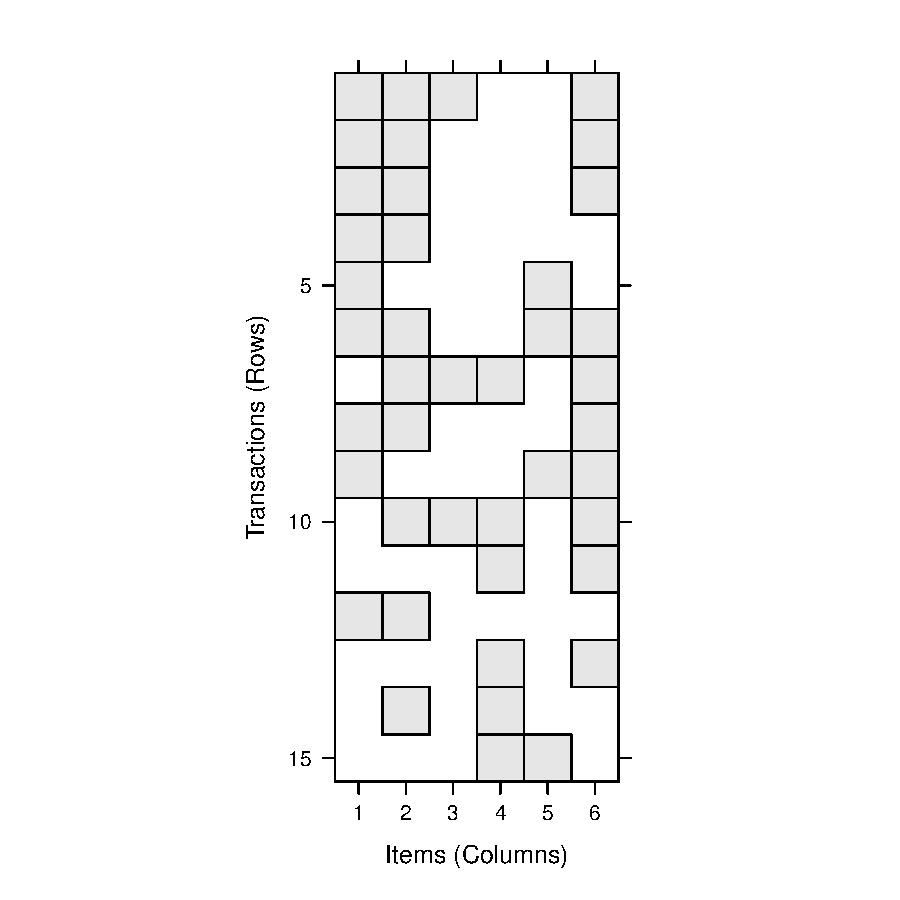
\includegraphics[width=.6\linewidth]{figure/ARULES1-SOLUCION-Rnwauto-report-1} 

}


\begin{kframe}\begin{alltt}
\hlcom{# Frecuencia relativa de los productos}
\hlkwd{itemFrequencyPlot}\hlstd{(trans,} \hlkwc{topN}\hlstd{=}\hlnum{10}\hlstd{,}  \hlkwc{cex.names}\hlstd{=}\hlnum{1}\hlstd{)}
\end{alltt}
\end{kframe}

{\centering 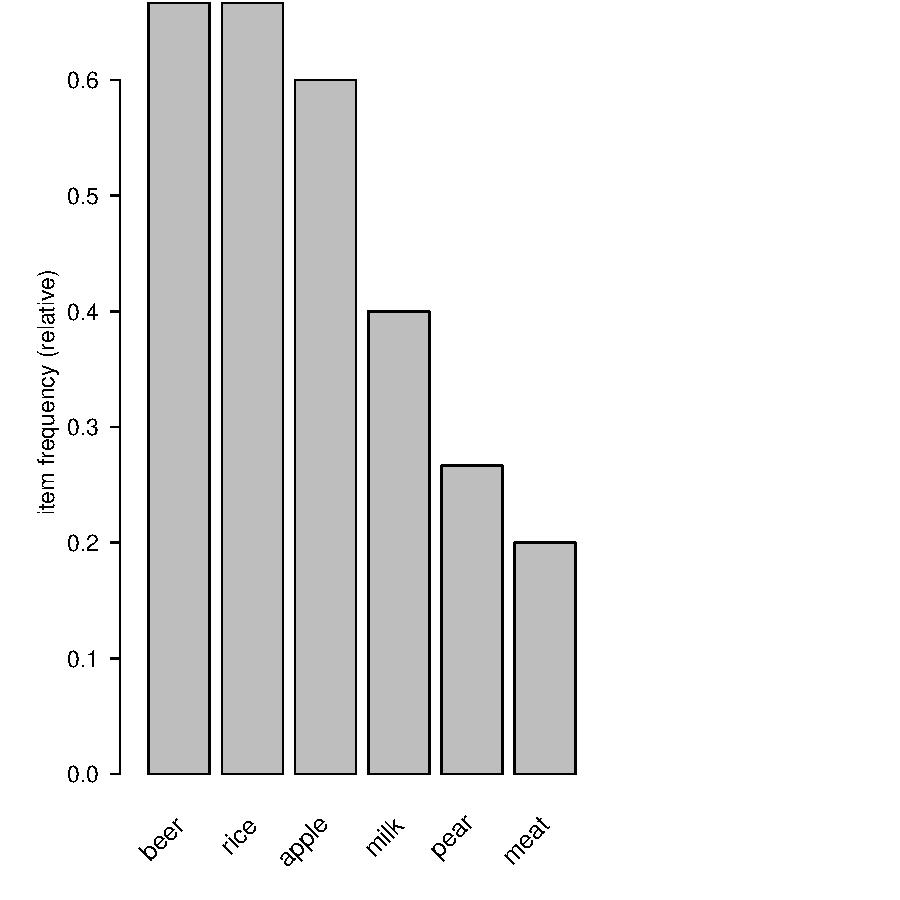
\includegraphics[width=.6\linewidth]{figure/ARULES1-SOLUCION-Rnwauto-report-2} 

}


\begin{kframe}\begin{alltt}
\hlcom{# A-Priori}

\hlcom{#Min Support 0.3, confidence 0.5.}
\hlstd{rules} \hlkwb{<-} \hlkwd{apriori}\hlstd{(trans,}
                 \hlkwc{parameter} \hlstd{=} \hlkwd{list}\hlstd{(}\hlkwc{supp}\hlstd{=}\hlnum{0.3}\hlstd{,} \hlkwc{conf}\hlstd{=}\hlnum{0.5}\hlstd{,}
                                  \hlkwc{maxlen}\hlstd{=}\hlnum{10}\hlstd{,}
                                  \hlkwc{target}\hlstd{=} \hlstr{"rules"}\hlstd{))}
\end{alltt}
\begin{verbatim}
## Apriori
## 
## Parameter specification:
##  confidence minval smax arem  aval originalSupport maxtime support minlen maxlen target
##         0.5    0.1    1 none FALSE            TRUE       5     0.3      1     10  rules
##   ext
##  TRUE
## 
## Algorithmic control:
##  filter tree heap memopt load sort verbose
##     0.1 TRUE TRUE  FALSE TRUE    2    TRUE
## 
## Absolute minimum support count: 4 
## 
## set item appearances ...[0 item(s)] done [0.00s].
## set transactions ...[6 item(s), 15 transaction(s)] done [0.00s].
## sorting and recoding items ... [4 item(s)] done [0.00s].
## creating transaction tree ... done [0.00s].
## checking subsets of size 1 2 3 done [0.00s].
## writing ... [12 rule(s)] done [0.00s].
## creating S4 object  ... done [0.00s].
\end{verbatim}
\begin{alltt}
\hlkwd{summary}\hlstd{(rules)}
\end{alltt}
\begin{verbatim}
## set of 12 rules
## 
## rule length distribution (lhs + rhs):sizes
## 1 2 3 
## 3 6 3 
## 
##    Min. 1st Qu.  Median    Mean 3rd Qu.    Max. 
##    1.00    1.75    2.00    2.00    2.25    3.00 
## 
## summary of quality measures:
##     support         confidence        coverage           lift           count      
##  Min.   :0.3333   Min.   :0.6000   Min.   :0.4000   Min.   :1.000   Min.   : 5.00  
##  1st Qu.:0.3833   1st Qu.:0.6667   1st Qu.:0.5667   1st Qu.:1.000   1st Qu.: 5.75  
##  Median :0.4667   Median :0.7000   Median :0.6667   Median :1.050   Median : 7.00  
##  Mean   :0.4667   Mean   :0.6950   Mean   :0.6833   Mean   :1.079   Mean   : 7.00  
##  3rd Qu.:0.5000   3rd Qu.:0.7143   3rd Qu.:0.7500   3rd Qu.:1.167   3rd Qu.: 7.50  
##  Max.   :0.6667   Max.   :0.8333   Max.   :1.0000   Max.   :1.250   Max.   :10.00  
## 
## mining info:
##   data ntransactions support confidence
##  trans            15     0.3        0.5
##                                                                                            call
##  apriori(data = trans, parameter = list(supp = 0.3, conf = 0.5, maxlen = 10, target = "rules"))
\end{verbatim}
\begin{alltt}
\hlcom{# Producto `beer`}
\hlstd{beer_rules_lhs} \hlkwb{<-} \hlkwd{apriori}\hlstd{(trans,}
                          \hlkwc{parameter} \hlstd{=} \hlkwd{list}\hlstd{(}\hlkwc{supp}\hlstd{=}\hlnum{0.3}\hlstd{,} \hlkwc{conf}\hlstd{=}\hlnum{0.5}\hlstd{,}
                                           \hlkwc{maxlen}\hlstd{=}\hlnum{10}\hlstd{,}
                                           \hlkwc{minlen}\hlstd{=}\hlnum{2}\hlstd{),}
                          \hlkwc{appearance} \hlstd{=} \hlkwd{list}\hlstd{(}\hlkwc{lhs}\hlstd{=}\hlstr{"beer"}\hlstd{,} \hlkwc{default}\hlstd{=}\hlstr{"rhs"}\hlstd{))}
\end{alltt}
\begin{verbatim}
## Apriori
## 
## Parameter specification:
##  confidence minval smax arem  aval originalSupport maxtime support minlen maxlen target
##         0.5    0.1    1 none FALSE            TRUE       5     0.3      2     10  rules
##   ext
##  TRUE
## 
## Algorithmic control:
##  filter tree heap memopt load sort verbose
##     0.1 TRUE TRUE  FALSE TRUE    2    TRUE
## 
## Absolute minimum support count: 4 
## 
## set item appearances ...[1 item(s)] done [0.00s].
## set transactions ...[6 item(s), 15 transaction(s)] done [0.00s].
## sorting and recoding items ... [4 item(s)] done [0.00s].
## creating transaction tree ... done [0.00s].
## checking subsets of size 1 2 done [0.00s].
## writing ... [2 rule(s)] done [0.00s].
## creating S4 object  ... done [0.00s].
\end{verbatim}
\begin{alltt}
\hlkwd{inspect}\hlstd{(beer_rules_lhs)}
\end{alltt}
\begin{verbatim}
##     lhs       rhs     support   confidence coverage  lift     count
## [1] {beer} => {apple} 0.4666667 0.7        0.6666667 1.166667 7    
## [2] {beer} => {rice}  0.4666667 0.7        0.6666667 1.050000 7
\end{verbatim}
\begin{alltt}
\hlcom{# Visualizar las reglas}
\hlstd{subrules} \hlkwb{<-} \hlkwd{head}\hlstd{(rules,} \hlkwc{n}\hlstd{=}\hlnum{10}\hlstd{,} \hlkwc{by} \hlstd{=} \hlstr{"confidence"}\hlstd{)}

\hlkwd{plot}\hlstd{(subrules,} \hlkwc{method} \hlstd{=} \hlstr{"graph"}\hlstd{,}  \hlkwc{engine} \hlstd{=} \hlstr{"htmlwidget"}\hlstd{)}
\end{alltt}


{\ttfamily\noindent\bfseries\color{errorcolor}{\#\# Error: package 'webshot' was installed before R 4.0.0: please re-install it}}\begin{alltt}
\hlkwd{plot}\hlstd{(subrules,} \hlkwc{method}\hlstd{=}\hlstr{"paracoord"}\hlstd{)}
\end{alltt}
\end{kframe}

{\centering 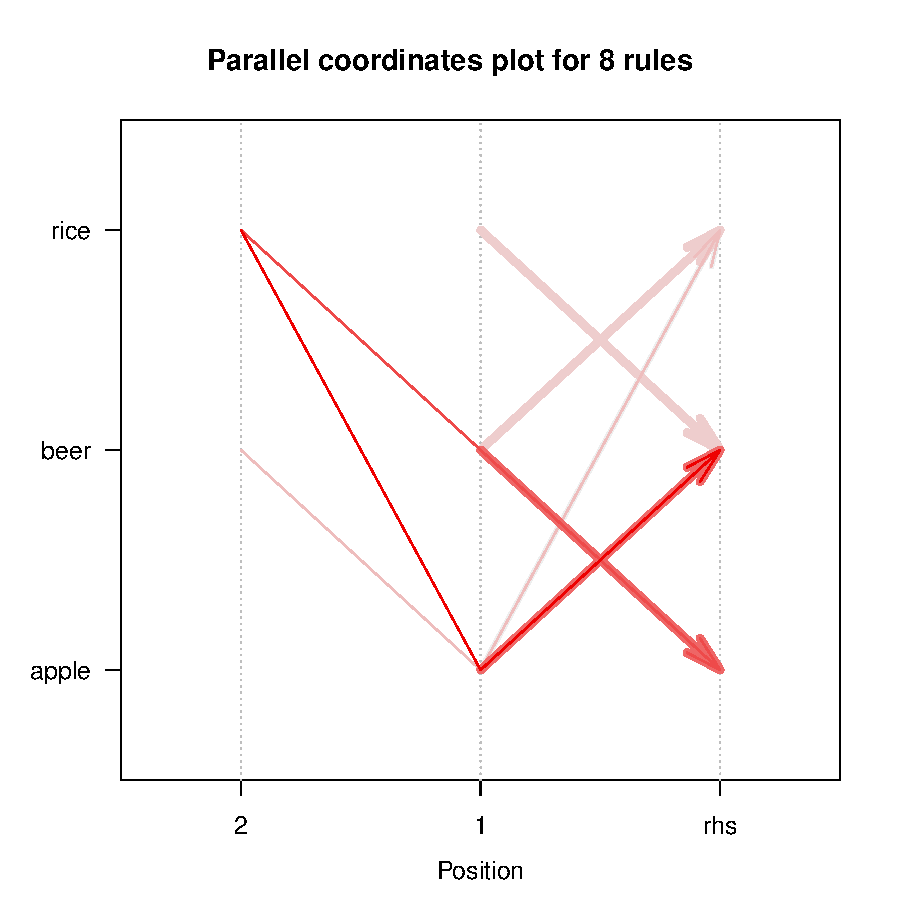
\includegraphics[width=.6\linewidth]{figure/ARULES1-SOLUCION-Rnwauto-report-3} 

}


\end{knitrout}

The R session information (including the OS info, R version and all
packages used):

\begin{knitrout}
\definecolor{shadecolor}{rgb}{0.969, 0.969, 0.969}\color{fgcolor}\begin{kframe}
\begin{alltt}
\hlkwd{sessionInfo}\hlstd{()}
\end{alltt}
\begin{verbatim}
## R version 4.3.1 (2023-06-16)
## Platform: x86_64-pc-linux-gnu (64-bit)
## Running under: Ubuntu 20.04.6 LTS
## 
## Matrix products: default
## BLAS:   /usr/lib/x86_64-linux-gnu/atlas/libblas.so.3.10.3 
## LAPACK: /usr/lib/x86_64-linux-gnu/atlas/liblapack.so.3.10.3;  LAPACK version 3.9.0
## 
## locale:
##  [1] LC_CTYPE=es_ES.UTF-8       LC_NUMERIC=C               LC_TIME=es_ES.UTF-8       
##  [4] LC_COLLATE=es_ES.UTF-8     LC_MONETARY=es_ES.UTF-8    LC_MESSAGES=es_ES.UTF-8   
##  [7] LC_PAPER=es_ES.UTF-8       LC_NAME=C                  LC_ADDRESS=C              
## [10] LC_TELEPHONE=C             LC_MEASUREMENT=es_ES.UTF-8 LC_IDENTIFICATION=C       
## 
## time zone: Europe/Madrid
## tzcode source: system (glibc)
## 
## attached base packages:
## [1] stats     graphics  grDevices utils     datasets  methods   base     
## 
## other attached packages:
##  [1] arulesViz_1.5-2  arules_1.7-6     Matrix_1.6-1.1   liver_1.15       ggfortify_0.4.16
##  [6] factoextra_1.0.7 mlbench_2.1-3.1  readxl_1.4.3     caret_6.0-94     lattice_0.21-9  
## [11] ggplot2_3.4.3    rpart.plot_3.1.1 rpart_4.1.19     caTools_1.18.2   dplyr_1.1.3     
## [16] ISLR2_1.3-2     
## 
## loaded via a namespace (and not attached):
##  [1] bitops_1.0-7         pROC_1.18.4          gridExtra_2.3        rlang_1.1.1         
##  [5] magrittr_2.0.3       e1071_1.7-13         compiler_4.3.1       vctrs_0.6.3         
##  [9] reshape2_1.4.4       stringr_1.5.0        pkgconfig_2.0.3      fastmap_1.1.1       
## [13] ellipsis_0.3.2       labeling_0.4.3       ggraph_2.1.0         utf8_1.2.3          
## [17] rmarkdown_2.25       prodlim_2023.08.28   tzdb_0.4.0           tinytex_0.47        
## [21] purrr_1.0.2          xfun_0.40            jsonlite_1.8.7       recipes_1.0.8       
## [25] highr_0.10           tweenr_2.0.2         parallel_4.3.1       R6_2.5.1            
## [29] stringi_1.7.12       parallelly_1.36.0    lubridate_1.9.3      cellranger_1.1.0    
## [33] Rcpp_1.0.11          iterators_1.0.14     knitr_1.44           future.apply_1.11.0 
## [37] readr_2.1.4          splines_4.3.1        nnet_7.3-19          igraph_1.5.1        
## [41] timechange_0.2.0     tidyselect_1.2.0     rstudioapi_0.15.0    yaml_2.3.7          
## [45] viridis_0.6.4        timeDate_4022.108    codetools_0.2-19     listenv_0.9.0       
## [49] tibble_3.2.1         plyr_1.8.9           withr_2.5.1          evaluate_0.22       
## [53] future_1.33.0        survival_3.5-7       proxy_0.4-27         polyclip_1.10-6     
## [57] pillar_1.9.0         foreach_1.5.2        stats4_4.3.1         generics_0.1.3      
## [61] hms_1.1.3            munsell_0.5.0        scales_1.2.1         globals_0.16.2      
## [65] class_7.3-22         glue_1.6.2           tools_4.3.1          data.table_1.14.8   
## [69] ModelMetrics_1.2.2.2 gower_1.0.1          visNetwork_2.1.2     graphlayouts_1.0.1  
## [73] tidygraph_1.2.3      grid_4.3.1           tidyr_1.3.0          ipred_0.9-14        
## [77] colorspace_2.1-0     nlme_3.1-163         ggforce_0.4.1        cli_3.6.1           
## [81] fansi_1.0.5          viridisLite_0.4.2    lava_1.7.2.1         gtable_0.3.4        
## [85] digest_0.6.33        ggrepel_0.9.3        htmlwidgets_1.6.2    farver_2.1.1        
## [89] htmltools_0.5.6.1    lifecycle_1.0.3      hardhat_1.3.0        MASS_7.3-60
\end{verbatim}
\begin{alltt}
\hlkwd{Sys.time}\hlstd{()}
\end{alltt}
\begin{verbatim}
## [1] "2023-11-02 18:33:30 CET"
\end{verbatim}
\end{kframe}
\end{knitrout}


\end{document}
